\documentclass{report}

\usepackage[a4paper,margin=0.5in]{geometry}
\usepackage{array}
\usepackage{xcolor}
\usepackage{graphicx}
\usepackage{float}

\newcolumntype{P}[1]{>{\raggedleft\arraybackslash}b{#1}}
\newcommand{\bftab}{\fontseries{b}\selectfont}

\begin{document}
\section{Plots of single attributes}

\subsection{quality}
\begin{figure}[H]
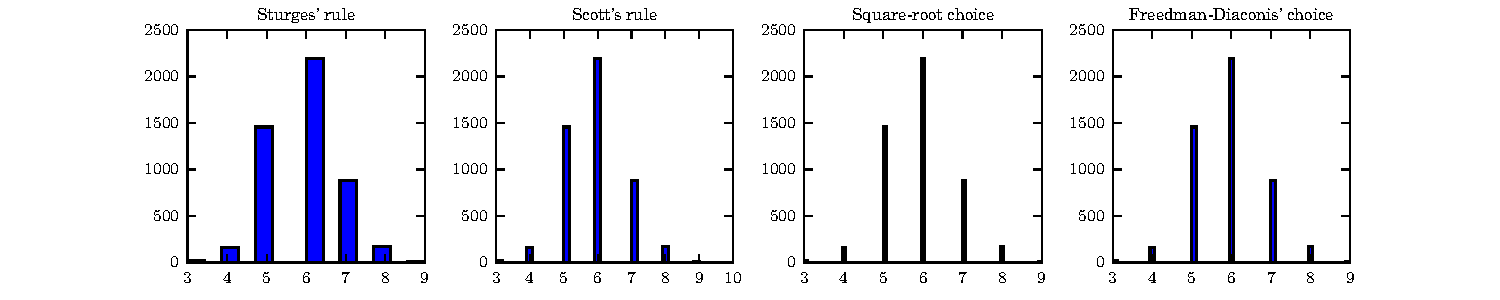
\includegraphics[width=\textwidth]{histograms/quality.pdf}
\caption{Histograms of attribute \emph{quality} using different binning methods}\end{figure}

\begin{figure}[H]
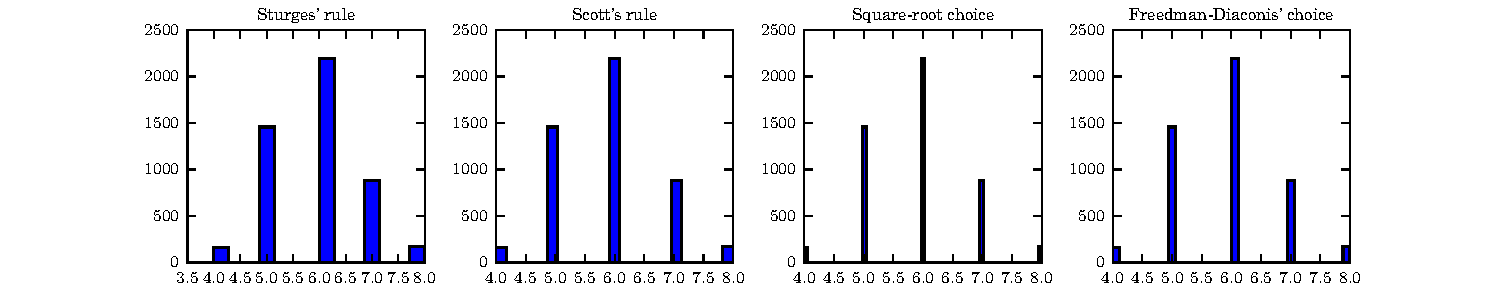
\includegraphics[width=\textwidth]{histograms/quality_filtered.pdf}
\caption{Histograms of attribute \emph{quality} with outliers further than 3 standard deviations from the mean filtered}\n\end{figure}

\begin{figure}[H]
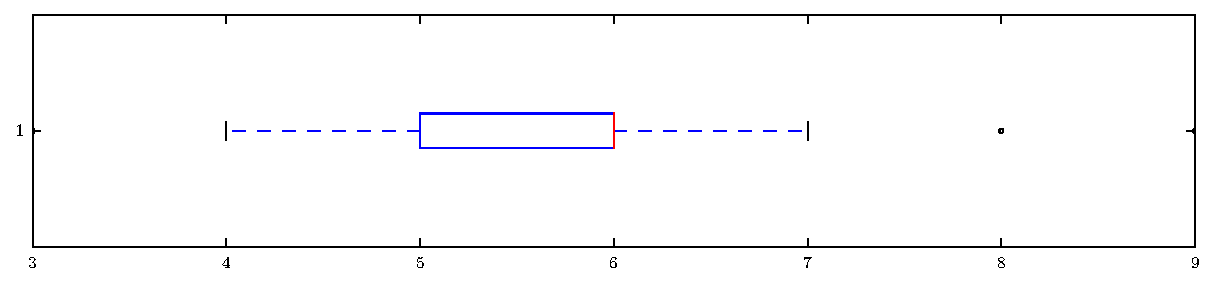
\includegraphics[width=\textwidth]{boxplots/quality.pdf}
\caption{Boxplot of attribute \emph{quality}}\end{figure}

\newpage\subsection{pH}
\begin{figure}[H]
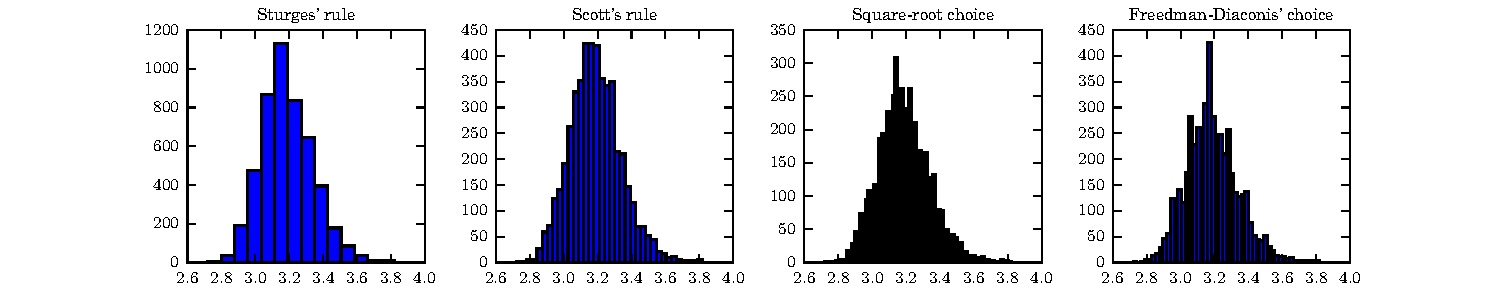
\includegraphics[width=\textwidth]{histograms/pH.pdf}
\caption{Histograms of attribute \emph{pH} using different binning methods}\end{figure}

\begin{figure}[H]
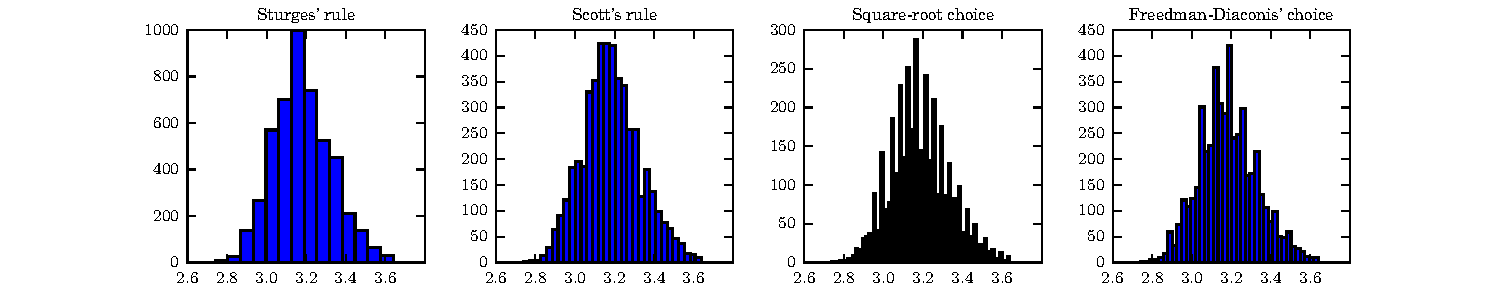
\includegraphics[width=\textwidth]{histograms/pH_filtered.pdf}
\caption{Histograms of attribute \emph{pH} with outliers further than 3 standard deviations from the mean filtered}\n\end{figure}

\begin{figure}[H]
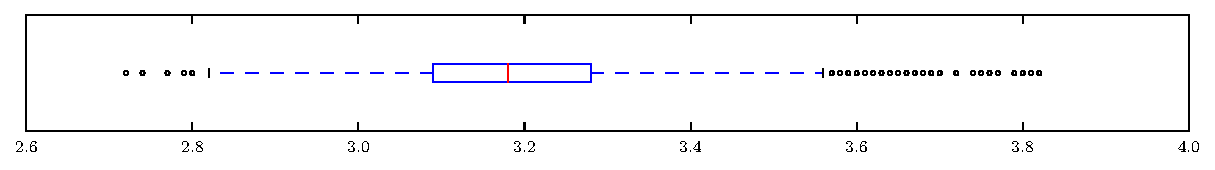
\includegraphics[width=\textwidth]{boxplots/pH.pdf}
\caption{Boxplot of attribute \emph{pH}}\end{figure}

\newpage\subsection{chlorides}
\begin{figure}[H]
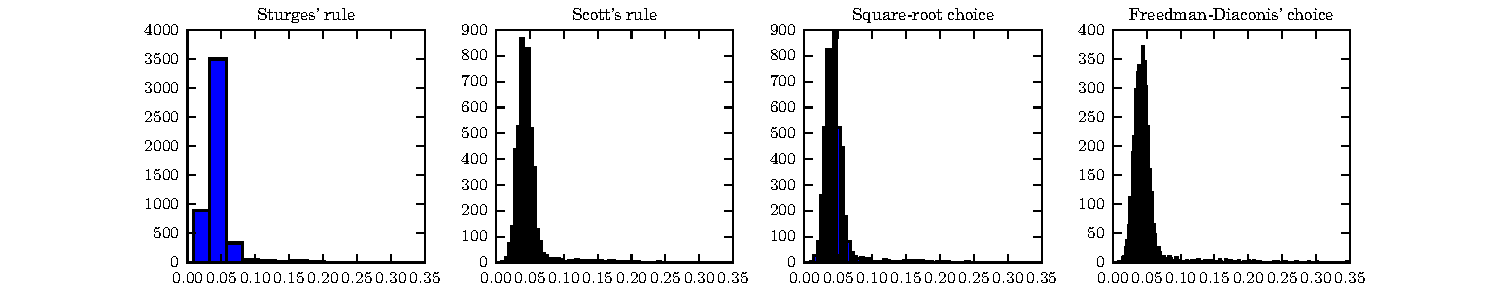
\includegraphics[width=\textwidth]{histograms/chlorides.pdf}
\caption{Histograms of attribute \emph{chlorides} using different binning methods}\end{figure}

\begin{figure}[H]
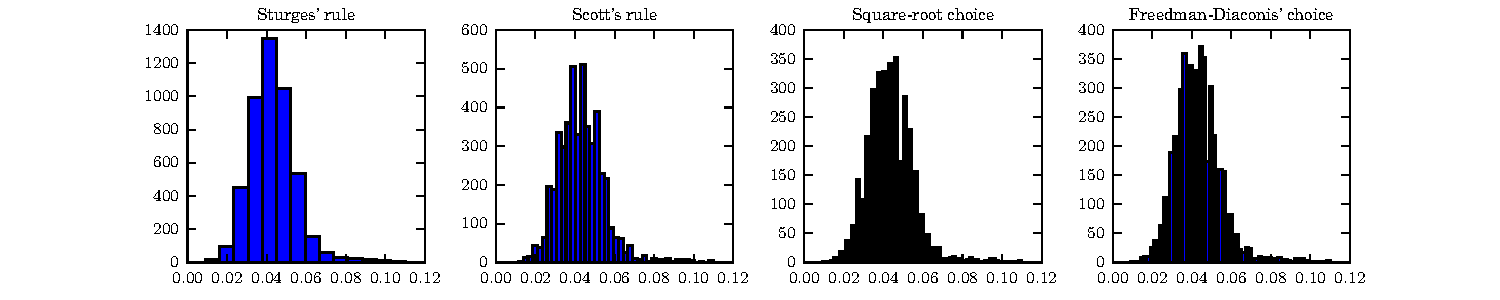
\includegraphics[width=\textwidth]{histograms/chlorides_filtered.pdf}
\caption{Histograms of attribute \emph{chlorides} with outliers further than 3 standard deviations from the mean filtered}\n\end{figure}

\begin{figure}[H]
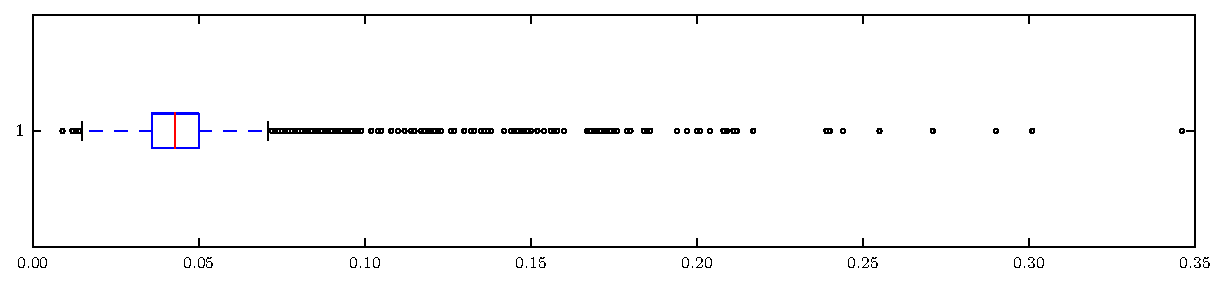
\includegraphics[width=\textwidth]{boxplots/chlorides.pdf}
\caption{Boxplot of attribute \emph{chlorides}}\end{figure}

\newpage\subsection{fixed acidity}
\begin{figure}[H]
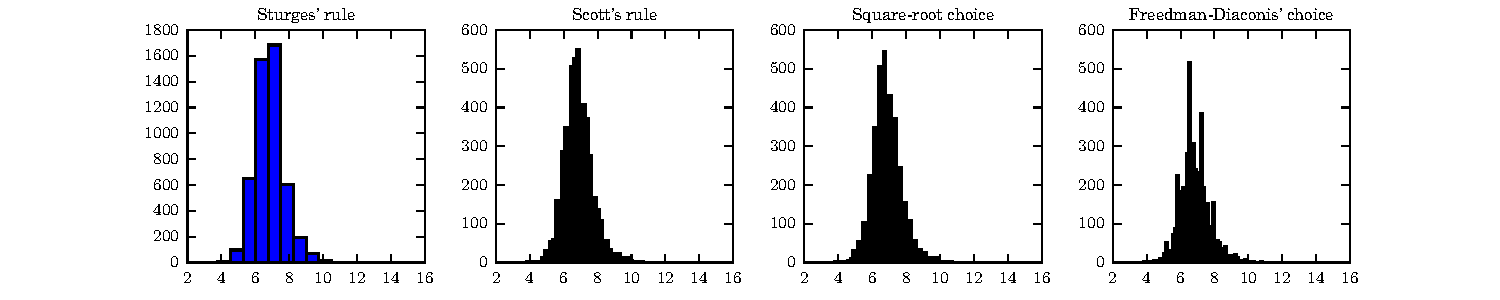
\includegraphics[width=\textwidth]{histograms/fixed_acidity.pdf}
\caption{Histograms of attribute \emph{fixed acidity} using different binning methods}\end{figure}

\begin{figure}[H]
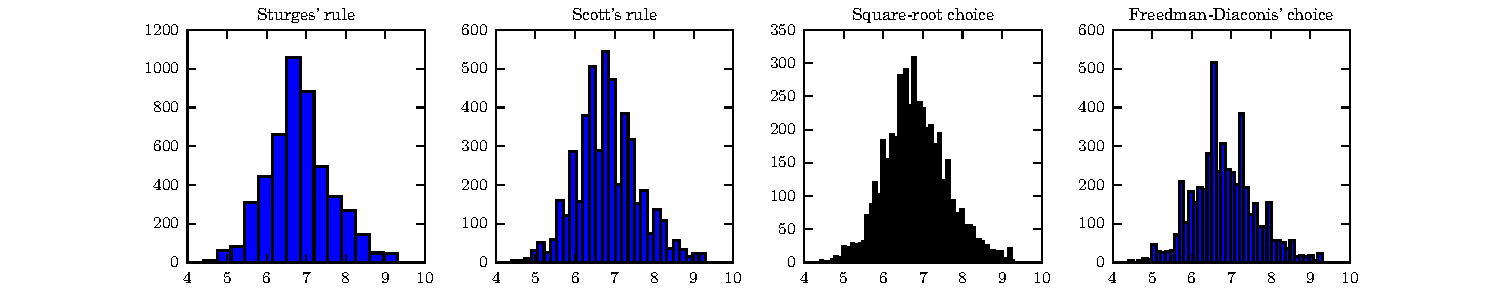
\includegraphics[width=\textwidth]{histograms/fixed_acidity_filtered.pdf}
\caption{Histograms of attribute \emph{fixed acidity} with outliers further than 3 standard deviations from the mean filtered}\n\end{figure}

\begin{figure}[H]
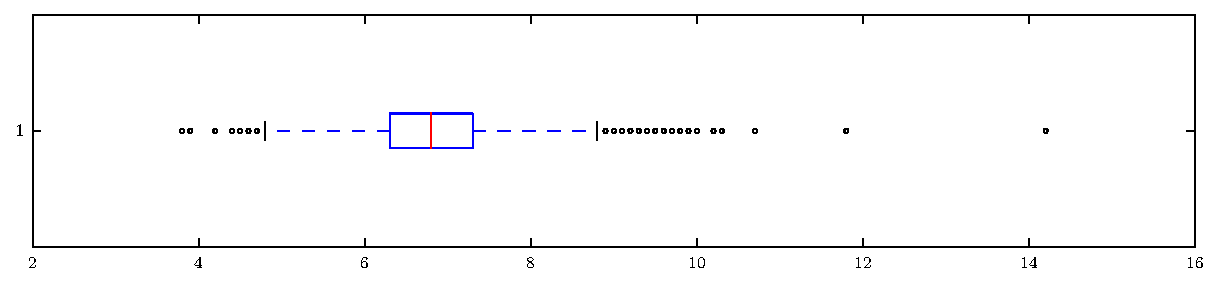
\includegraphics[width=\textwidth]{boxplots/fixed_acidity.pdf}
\caption{Boxplot of attribute \emph{fixed acidity}}\end{figure}

\newpage\subsection{density}
\begin{figure}[H]
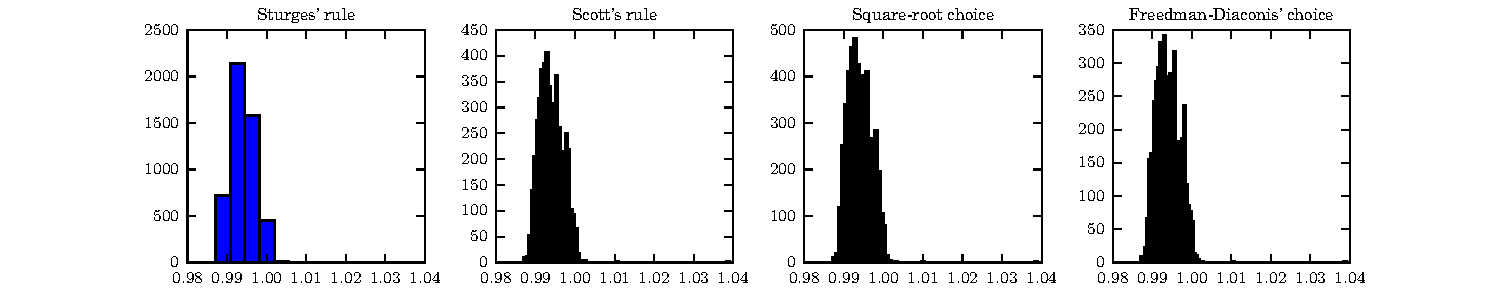
\includegraphics[width=\textwidth]{histograms/density.pdf}
\caption{Histograms of attribute \emph{density} using different binning methods}\end{figure}

\begin{figure}[H]
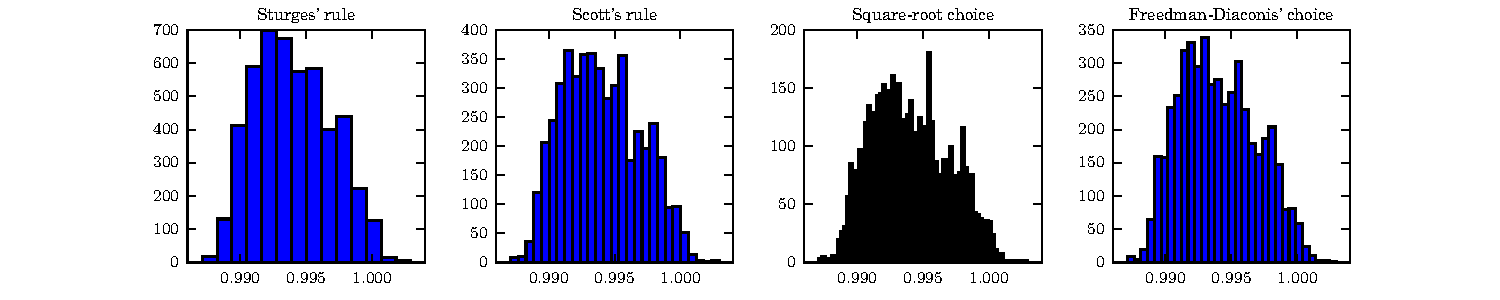
\includegraphics[width=\textwidth]{histograms/density_filtered.pdf}
\caption{Histograms of attribute \emph{density} with outliers further than 3 standard deviations from the mean filtered}\n\end{figure}

\begin{figure}[H]
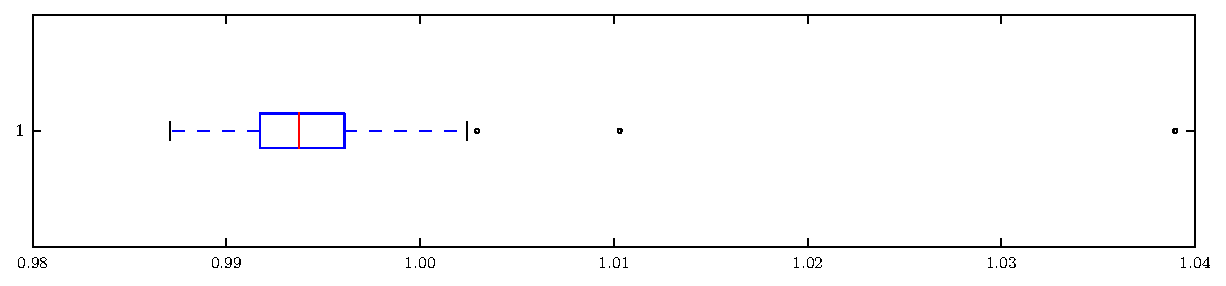
\includegraphics[width=\textwidth]{boxplots/density.pdf}
\caption{Boxplot of attribute \emph{density}}\end{figure}

\newpage\subsection{residual sugar}
\begin{figure}[H]
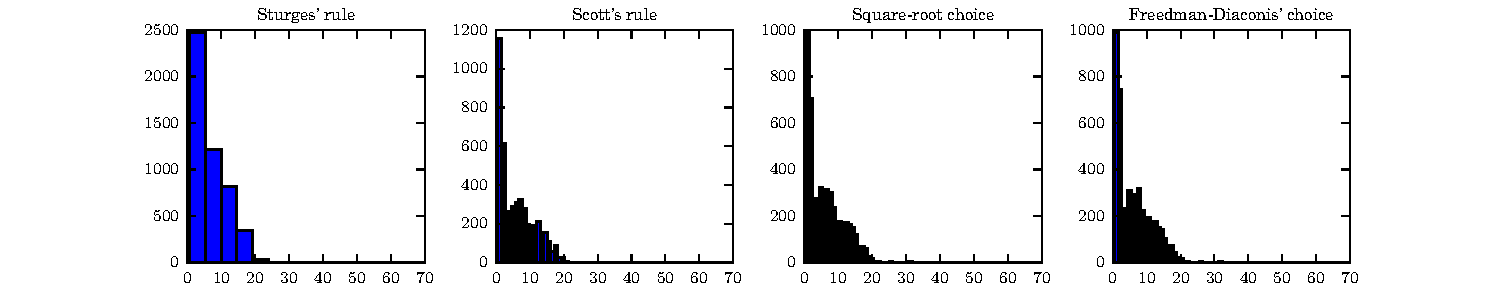
\includegraphics[width=\textwidth]{histograms/residual_sugar.pdf}
\caption{Histograms of attribute \emph{residual sugar} using different binning methods}\end{figure}

\begin{figure}[H]
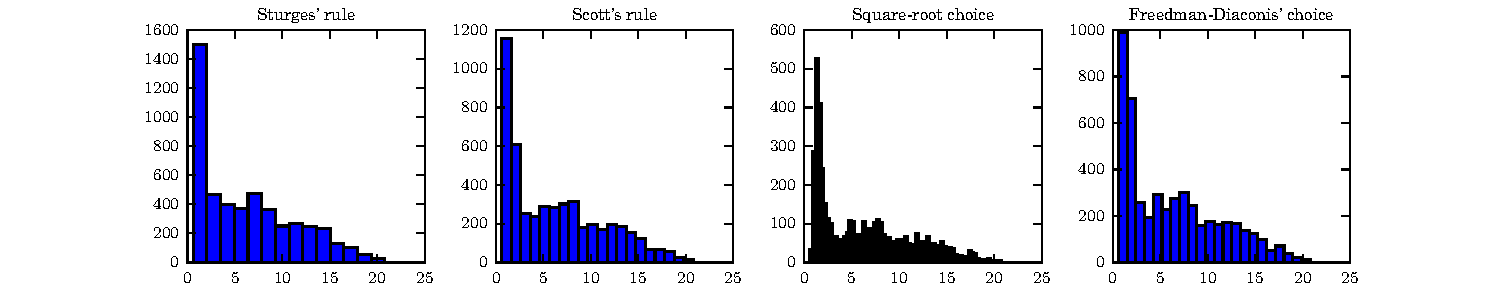
\includegraphics[width=\textwidth]{histograms/residual_sugar_filtered.pdf}
\caption{Histograms of attribute \emph{residual sugar} with outliers further than 3 standard deviations from the mean filtered}\n\end{figure}

\begin{figure}[H]
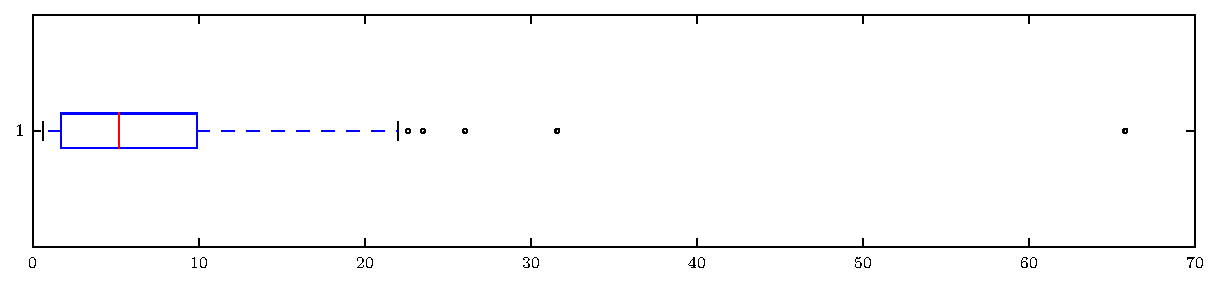
\includegraphics[width=\textwidth]{boxplots/residual_sugar.pdf}
\caption{Boxplot of attribute \emph{residual sugar}}\end{figure}

\newpage\subsection{total sulfur dioxide}
\begin{figure}[H]
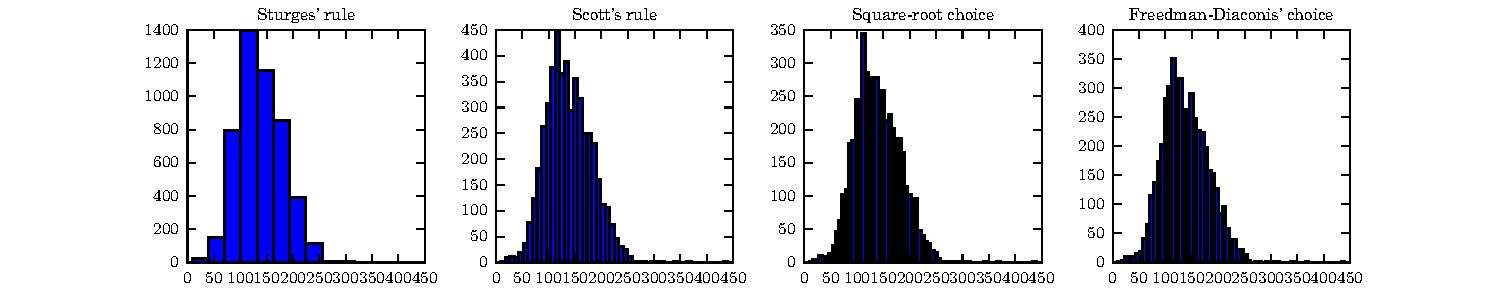
\includegraphics[width=\textwidth]{histograms/total_sulfur_dioxide.pdf}
\caption{Histograms of attribute \emph{total sulfur dioxide} using different binning methods}\end{figure}

\begin{figure}[H]
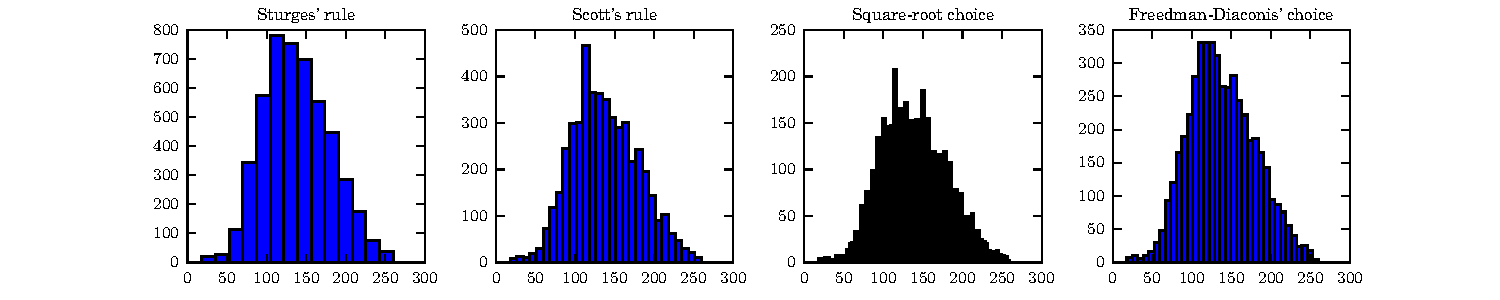
\includegraphics[width=\textwidth]{histograms/total_sulfur_dioxide_filtered.pdf}
\caption{Histograms of attribute \emph{total sulfur dioxide} with outliers further than 3 standard deviations from the mean filtered}\n\end{figure}

\begin{figure}[H]
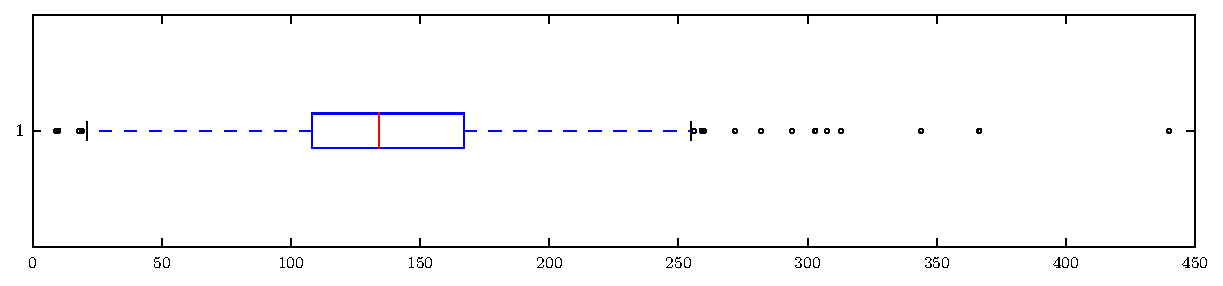
\includegraphics[width=\textwidth]{boxplots/total_sulfur_dioxide.pdf}
\caption{Boxplot of attribute \emph{total sulfur dioxide}}\end{figure}

\newpage\subsection{citric acid}
\begin{figure}[H]
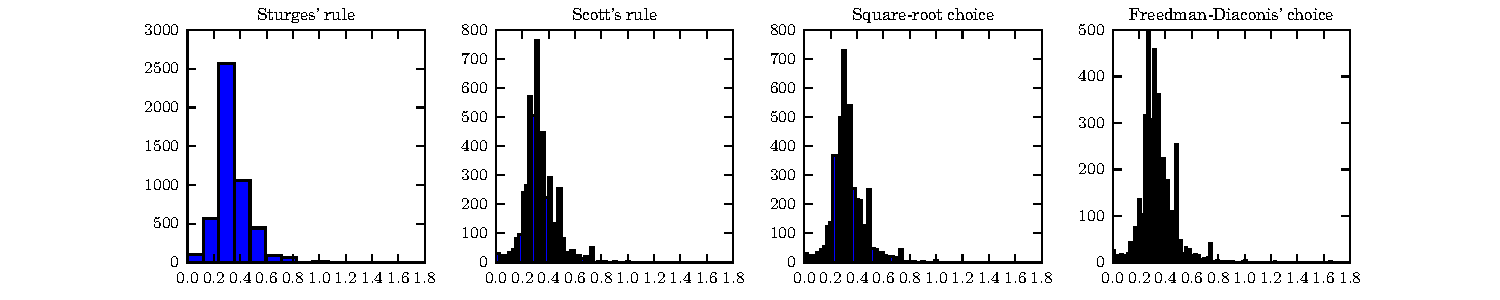
\includegraphics[width=\textwidth]{histograms/citric_acid.pdf}
\caption{Histograms of attribute \emph{citric acid} using different binning methods}\end{figure}

\begin{figure}[H]
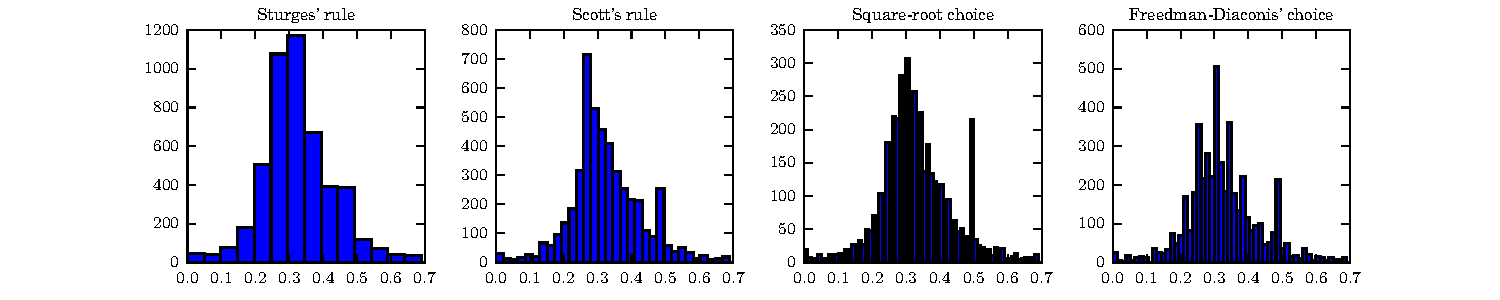
\includegraphics[width=\textwidth]{histograms/citric_acid_filtered.pdf}
\caption{Histograms of attribute \emph{citric acid} with outliers further than 3 standard deviations from the mean filtered}\n\end{figure}

\begin{figure}[H]
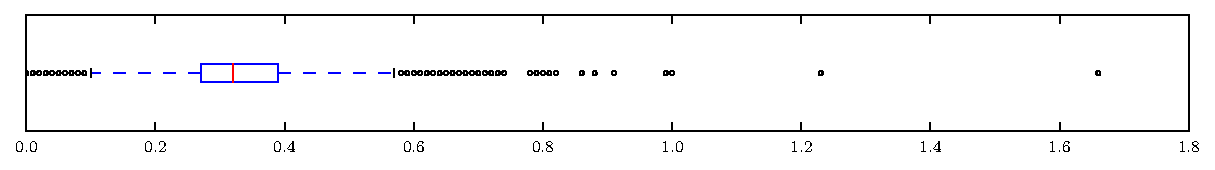
\includegraphics[width=\textwidth]{boxplots/citric_acid.pdf}
\caption{Boxplot of attribute \emph{citric acid}}\end{figure}

\newpage\subsection{volatile acidity}
\begin{figure}[H]
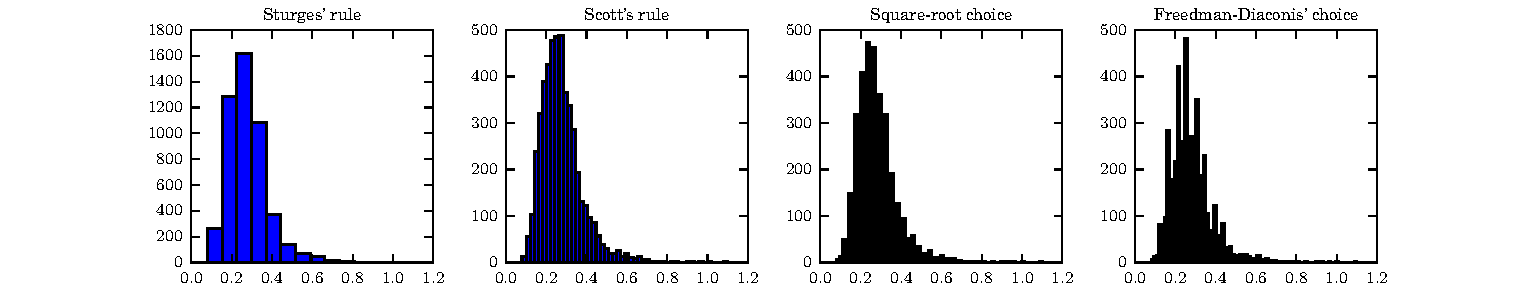
\includegraphics[width=\textwidth]{histograms/volatile_acidity.pdf}
\caption{Histograms of attribute \emph{volatile acidity} using different binning methods}\end{figure}

\begin{figure}[H]
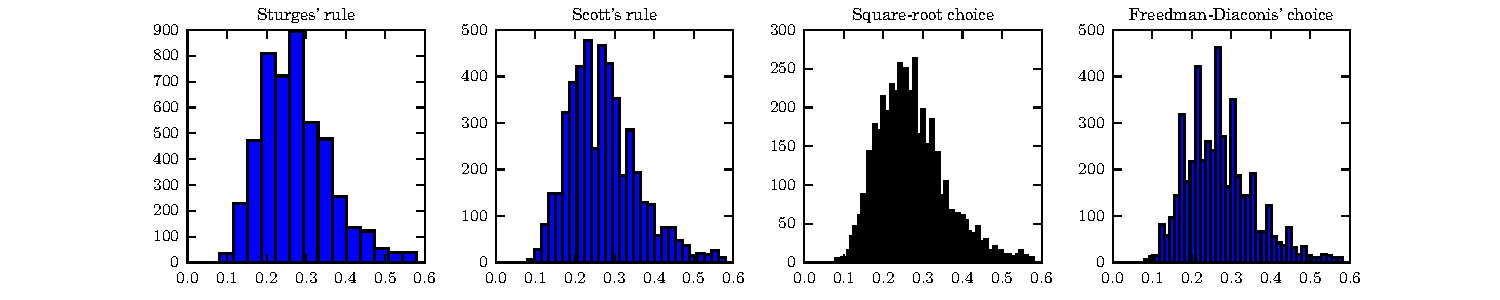
\includegraphics[width=\textwidth]{histograms/volatile_acidity_filtered.pdf}
\caption{Histograms of attribute \emph{volatile acidity} with outliers further than 3 standard deviations from the mean filtered}\n\end{figure}

\begin{figure}[H]
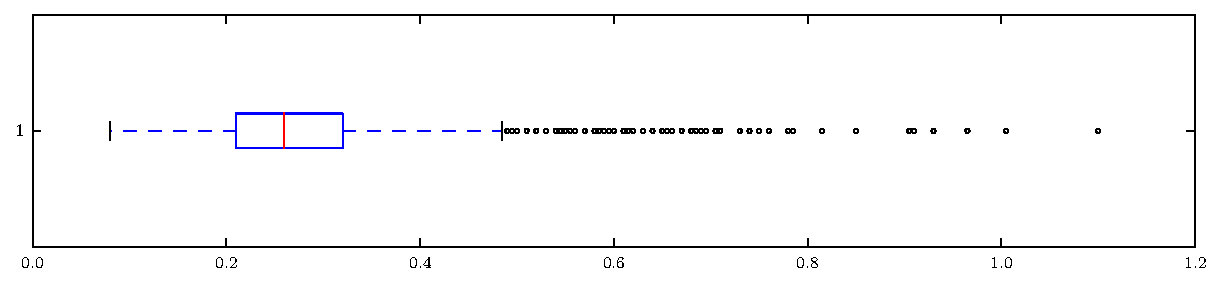
\includegraphics[width=\textwidth]{boxplots/volatile_acidity.pdf}
\caption{Boxplot of attribute \emph{volatile acidity}}\end{figure}

\newpage\subsection{free sulfur dioxide}
\begin{figure}[H]
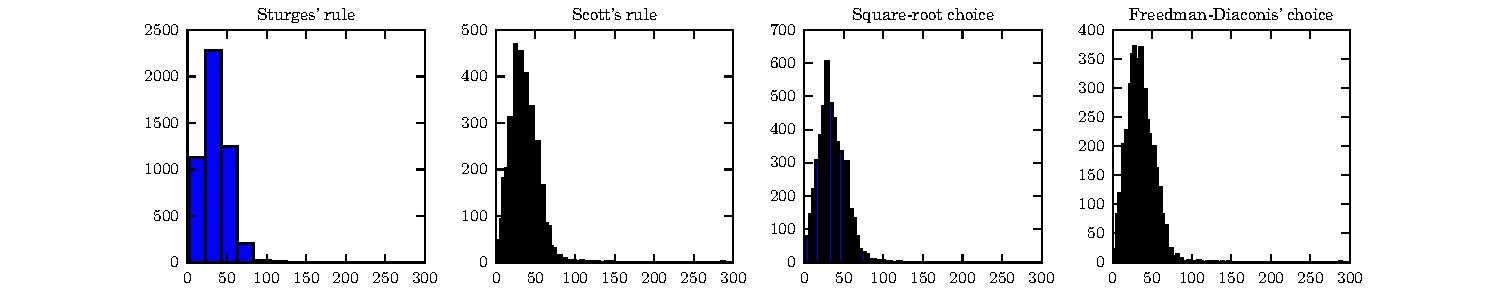
\includegraphics[width=\textwidth]{histograms/free_sulfur_dioxide.pdf}
\caption{Histograms of attribute \emph{free sulfur dioxide} using different binning methods}\end{figure}

\begin{figure}[H]
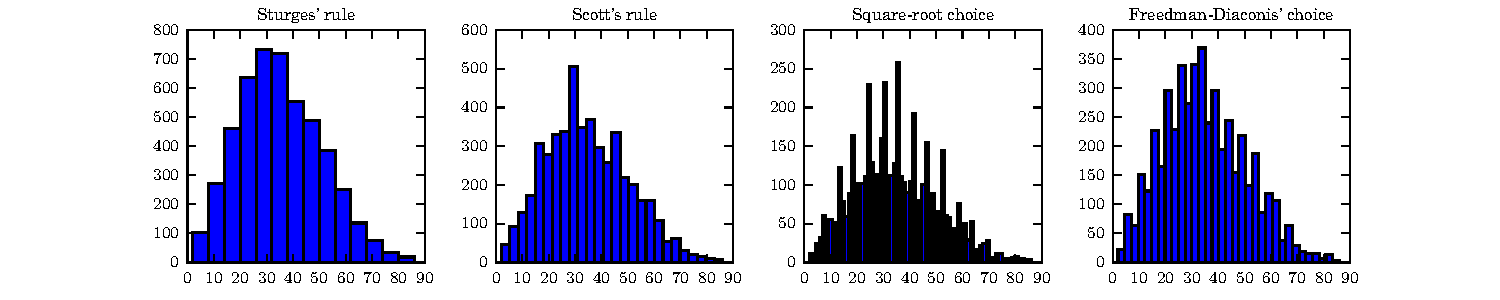
\includegraphics[width=\textwidth]{histograms/free_sulfur_dioxide_filtered.pdf}
\caption{Histograms of attribute \emph{free sulfur dioxide} with outliers further than 3 standard deviations from the mean filtered}\n\end{figure}

\begin{figure}[H]
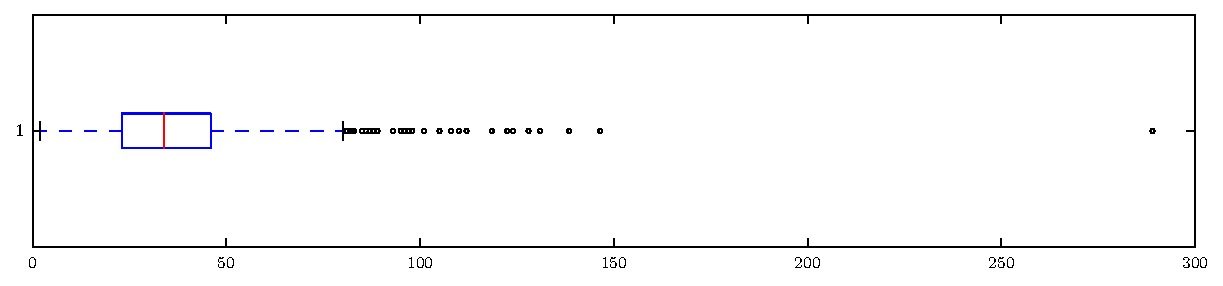
\includegraphics[width=\textwidth]{boxplots/free_sulfur_dioxide.pdf}
\caption{Boxplot of attribute \emph{free sulfur dioxide}}\end{figure}

\newpage\subsection{sulphates}
\begin{figure}[H]
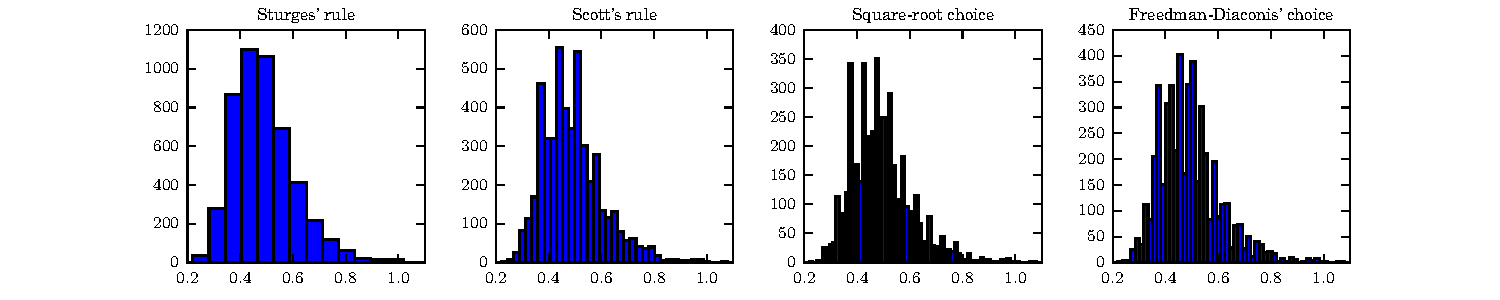
\includegraphics[width=\textwidth]{histograms/sulphates.pdf}
\caption{Histograms of attribute \emph{sulphates} using different binning methods}\end{figure}

\begin{figure}[H]
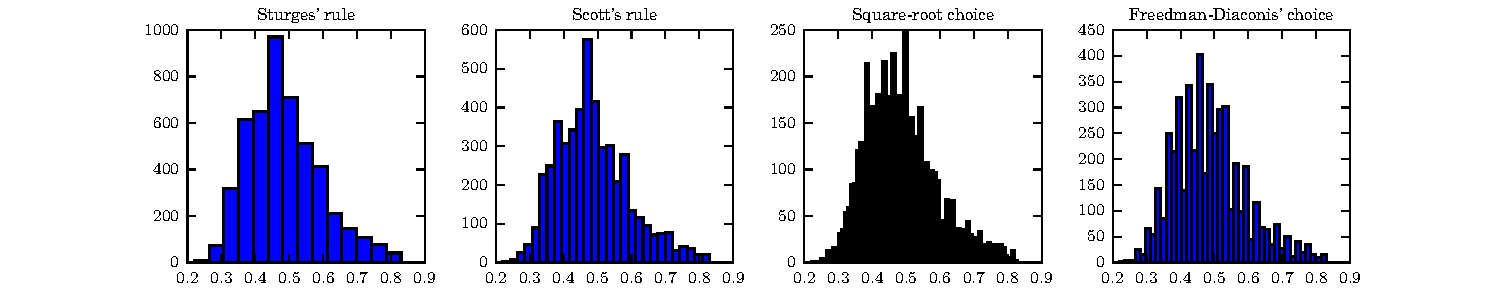
\includegraphics[width=\textwidth]{histograms/sulphates_filtered.pdf}
\caption{Histograms of attribute \emph{sulphates} with outliers further than 3 standard deviations from the mean filtered}\n\end{figure}

\begin{figure}[H]
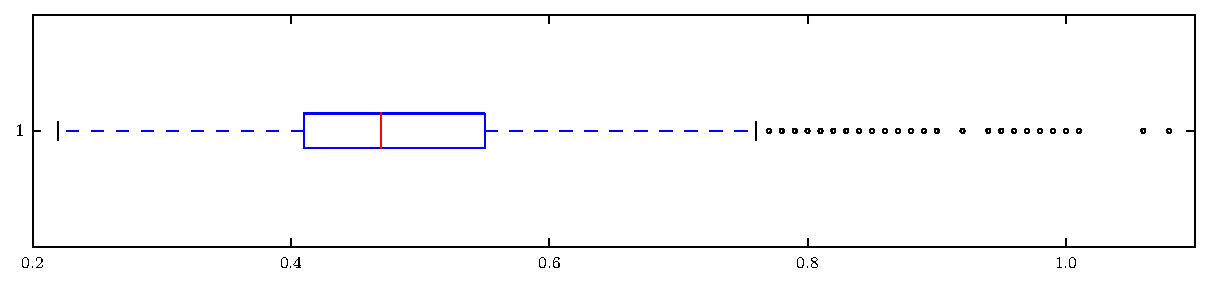
\includegraphics[width=\textwidth]{boxplots/sulphates.pdf}
\caption{Boxplot of attribute \emph{sulphates}}\end{figure}

\newpage\subsection{alcohol}
\begin{figure}[H]
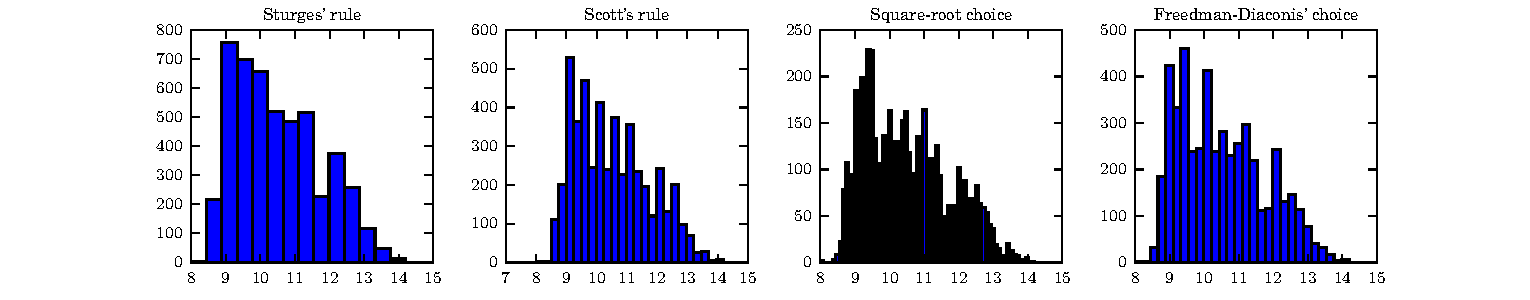
\includegraphics[width=\textwidth]{histograms/alcohol.pdf}
\caption{Histograms of attribute \emph{alcohol} using different binning methods}\end{figure}

\begin{figure}[H]
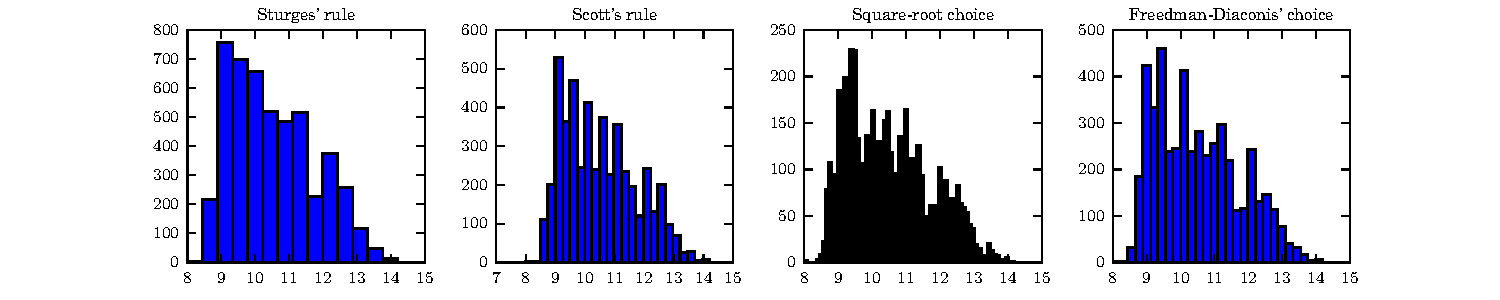
\includegraphics[width=\textwidth]{histograms/alcohol_filtered.pdf}
\caption{Histograms of attribute \emph{alcohol} with outliers further than 3 standard deviations from the mean filtered}\n\end{figure}

\begin{figure}[H]
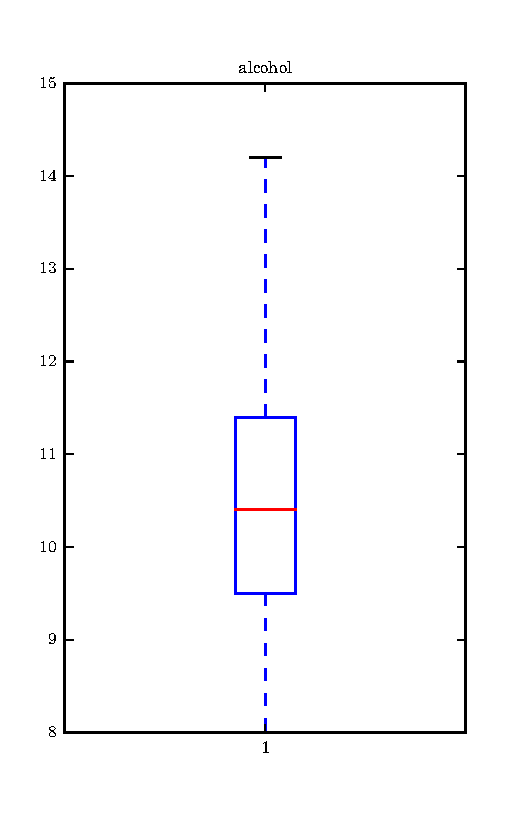
\includegraphics[width=\textwidth]{boxplots/alcohol.pdf}
\caption{Boxplot of attribute \emph{alcohol}}\end{figure}

\newpage\section{Correlation coefficients using different functions}

\subsection{Correlation coefficients using Pearson's correlation coefficient}
\begin{tabular}{l || *{12}{P{1.2cm}}}
& quality & pH & chlorides & fixed acidity & density & residual sugar & total sulfur dioxide & citric acid & volatile acidity & free sulfur dioxide & sulphates & alcohol\\
\hline 
quality & \bftab 1.0000 & 0.0994 & -0.2099 & -0.1137 & -0.3071 & -0.0976 & -0.1747 & -0.0092 & -0.1947 & 0.0082 & 0.0537 & 0.4356 \\

pH & 0.0994 & \bftab 1.0000 & -0.0904 & -0.4259 & -0.0936 & -0.1941 & 0.0023 & -0.1637 & -0.0319 & -0.0006 & 0.1560 & 0.1214 \\

chlorides & -0.2099 & -0.0904 & \bftab 1.0000 & 0.0231 & 0.2572 & 0.0887 & 0.1989 & 0.1144 & 0.0705 & 0.1014 & 0.0168 & -0.3602 \\

fixed acidity & -0.1137 & -0.4259 & 0.0231 & \bftab 1.0000 & 0.2653 & 0.0890 & 0.0911 & 0.2892 & -0.0227 & -0.0494 & -0.0171 & -0.1209 \\

density & -0.3071 & -0.0936 & 0.2572 & 0.2653 & \bftab 1.0000 & \bftab 0.8390 & \bftab 0.5299 & 0.1495 & 0.0271 & 0.2942 & 0.0745 & \bftab -0.7801 \\

residual sugar & -0.0976 & -0.1941 & 0.0887 & 0.0890 & \bftab 0.8390 & \bftab 1.0000 & 0.4014 & 0.0942 & 0.0643 & 0.2991 & -0.0267 & -0.4506 \\

total sulfur dioxide & -0.1747 & 0.0023 & 0.1989 & 0.0911 & \bftab 0.5299 & 0.4014 & \bftab 1.0000 & 0.1211 & 0.0893 & \bftab 0.6155 & 0.1346 & -0.4489 \\

citric acid & -0.0092 & -0.1637 & 0.1144 & 0.2892 & 0.1495 & 0.0942 & 0.1211 & \bftab 1.0000 & -0.1495 & 0.0941 & 0.0623 & -0.0757 \\

volatile acidity & -0.1947 & -0.0319 & 0.0705 & -0.0227 & 0.0271 & 0.0643 & 0.0893 & -0.1495 & \bftab 1.0000 & -0.0970 & -0.0357 & 0.0677 \\

free sulfur dioxide & 0.0082 & -0.0006 & 0.1014 & -0.0494 & 0.2942 & 0.2991 & \bftab 0.6155 & 0.0941 & -0.0970 & \bftab 1.0000 & 0.0592 & -0.2501 \\

sulphates & 0.0537 & 0.1560 & 0.0168 & -0.0171 & 0.0745 & -0.0267 & 0.1346 & 0.0623 & -0.0357 & 0.0592 & \bftab 1.0000 & -0.0174 \\

alcohol & 0.4356 & 0.1214 & -0.3602 & -0.1209 & \bftab -0.7801 & -0.4506 & -0.4489 & -0.0757 & 0.0677 & -0.2501 & -0.0174 & \bftab 1.0000 \\
\end{tabular}

\subsection{Correlation coefficients using Spearman's rho}
\begin{tabular}{l || *{12}{P{1.2cm}}}
& quality & pH & chlorides & fixed acidity & density & residual sugar & total sulfur dioxide & citric acid & volatile acidity & free sulfur dioxide & sulphates & alcohol\\
\hline 
quality & \bftab 1.0000 & 0.1094 & -0.3145 & -0.0845 & -0.3484 & -0.0821 & -0.1967 & 0.0183 & -0.1966 & 0.0237 & 0.0333 & 0.4404 \\

pH & 0.1094 & \bftab 1.0000 & -0.0540 & -0.4183 & -0.1101 & -0.1800 & -0.0118 & -0.1462 & -0.0452 & -0.0063 & 0.1402 & 0.1489 \\

chlorides & -0.3145 & -0.0540 & \bftab 1.0000 & 0.0947 & \bftab 0.5083 & 0.2278 & 0.3752 & 0.0327 & -0.0049 & 0.1670 & 0.0939 & \bftab -0.5708 \\

fixed acidity & -0.0845 & -0.4183 & 0.0947 & \bftab 1.0000 & 0.2700 & 0.1067 & 0.1126 & 0.2979 & -0.0429 & -0.0245 & -0.0132 & -0.1068 \\

density & -0.3484 & -0.1101 & \bftab 0.5083 & 0.2700 & \bftab 1.0000 & \bftab 0.7804 & \bftab 0.5638 & 0.0914 & 0.0101 & 0.3278 & 0.0951 & \bftab -0.8219 \\

residual sugar & -0.0821 & -0.1800 & 0.2278 & 0.1067 & \bftab 0.7804 & \bftab 1.0000 & 0.4313 & 0.0246 & 0.1086 & 0.3461 & -0.0038 & -0.4453 \\

total sulfur dioxide & -0.1967 & -0.0118 & 0.3752 & 0.1126 & \bftab 0.5638 & 0.4313 & \bftab 1.0000 & 0.0932 & 0.1176 & \bftab 0.6186 & 0.1578 & -0.4766 \\

citric acid & 0.0183 & -0.1462 & 0.0327 & 0.2979 & 0.0914 & 0.0246 & 0.0932 & \bftab 1.0000 & -0.1504 & 0.0883 & 0.0798 & -0.0292 \\

volatile acidity & -0.1966 & -0.0452 & -0.0049 & -0.0429 & 0.0101 & 0.1086 & 0.1176 & -0.1504 & \bftab 1.0000 & -0.0812 & -0.0169 & 0.0340 \\

free sulfur dioxide & 0.0237 & -0.0063 & 0.1670 & -0.0245 & 0.3278 & 0.3461 & \bftab 0.6186 & 0.0883 & -0.0812 & \bftab 1.0000 & 0.0523 & -0.2726 \\

sulphates & 0.0333 & 0.1402 & 0.0939 & -0.0132 & 0.0951 & -0.0038 & 0.1578 & 0.0798 & -0.0169 & 0.0523 & \bftab 1.0000 & -0.0449 \\

alcohol & 0.4404 & 0.1489 & \bftab -0.5708 & -0.1068 & \bftab -0.8219 & -0.4453 & -0.4766 & -0.0292 & 0.0340 & -0.2726 & -0.0449 & \bftab 1.0000 \\
\end{tabular}

\subsection{Correlation coefficients using Kendall's tau}
\begin{tabular}{l || *{12}{P{1.2cm}}}
& quality & pH & chlorides & fixed acidity & density & residual sugar & total sulfur dioxide & citric acid & volatile acidity & free sulfur dioxide & sulphates & alcohol\\
\hline 
quality & \bftab 1.0000 & 0.0844 & -0.2449 & -0.0655 & -0.2666 & -0.0631 & -0.1512 & 0.0146 & -0.1548 & 0.0172 & 0.0264 & 0.3467 \\

pH & 0.0844 & \bftab 1.0000 & -0.0379 & -0.2948 & -0.0756 & -0.1256 & -0.0084 & -0.1013 & -0.0304 & -0.0052 & 0.0958 & 0.1026 \\

chlorides & -0.2449 & -0.0379 & \bftab 1.0000 & 0.0654 & 0.3491 & 0.1553 & 0.2571 & 0.0223 & -0.0035 & 0.1139 & 0.0626 & -0.4040 \\

fixed acidity & -0.0655 & -0.2948 & 0.0654 & \bftab 1.0000 & 0.1855 & 0.0749 & 0.0773 & 0.2086 & -0.0296 & -0.0169 & -0.0087 & -0.0732 \\

density & -0.2666 & -0.0756 & 0.3491 & 0.1855 & \bftab 1.0000 & \bftab 0.5890 & 0.3884 & 0.0615 & 0.0066 & 0.2173 & 0.0642 & \bftab -0.6351 \\

residual sugar & -0.0631 & -0.1256 & 0.1553 & 0.0749 & \bftab 0.5890 & \bftab 1.0000 & 0.2933 & 0.0153 & 0.0728 & 0.2367 & -0.0025 & -0.3056 \\

total sulfur dioxide & -0.1512 & -0.0084 & 0.2571 & 0.0773 & 0.3884 & 0.2933 & \bftab 1.0000 & 0.0622 & 0.0813 & 0.4447 & 0.1087 & -0.3258 \\

citric acid & 0.0146 & -0.1013 & 0.0223 & 0.2086 & 0.0615 & 0.0153 & 0.0622 & \bftab 1.0000 & -0.1040 & 0.0608 & 0.0545 & -0.0200 \\

volatile acidity & -0.1548 & -0.0304 & -0.0035 & -0.0296 & 0.0066 & 0.0728 & 0.0813 & -0.1040 & \bftab 1.0000 & -0.0548 & -0.0116 & 0.0235 \\

free sulfur dioxide & 0.0172 & -0.0052 & 0.1139 & -0.0169 & 0.2173 & 0.2367 & 0.4447 & 0.0608 & -0.0548 & \bftab 1.0000 & 0.0356 & -0.1825 \\

sulphates & 0.0264 & 0.0958 & 0.0626 & -0.0087 & 0.0642 & -0.0025 & 0.1087 & 0.0545 & -0.0116 & 0.0356 & \bftab 1.0000 & -0.0264 \\

alcohol & 0.3467 & 0.1026 & -0.4040 & -0.0732 & \bftab -0.6351 & -0.3056 & -0.3258 & -0.0200 & 0.0235 & -0.1825 & -0.0264 & \bftab 1.0000 \\
\end{tabular}

\end{document}